\chapter{Sección Administrativa}

Esta sección aborda los aspectos administrativos que permiten una gestión integral y ordenada de todos los elementos de \textbf{QuickContentMedia}. 

\section{Codificación}

A continuación se especifican las directrices para la asignación de nombres y códigos a los distintos componentes del sistema de \textbf{QuickContentMedia}.

\subsection{Requisitos}
Los requisitos son codificados con la letra R seguida de la primera letra de las palabras si es funcional o no funcional y se les asigna un número único y secuencial.

%%%%%%%%%%%%%%%%%%% TABLA %%%%%%%%%%%%%%%%%%% 
\renewcommand{\arraystretch}{1.3} % para mejor espaciado vertical
\begin{longtable}{|c|c|}
\caption{Codificación de Requisitos} \\
\hline
\textbf{Código} & \textbf{Nombre} \\
\hline
\endfirsthead

\multicolumn{2}{c}%
{{\bfseries \tablename\ \thetable{} -- continuación desde la página anterior}} \\
\hline
\textbf{Código} & \textbf{Nombre} \\
\hline
\endhead

\hline \multicolumn{2}{r}{{Continúa en la siguiente página}} \\
\endfoot

\hline
\endlastfoot

%%%%%%%%%%%%%%%%%%%
RF-001 & Ingreso al portal \\
\hline

%%%%%%%%%%%%%%%%%%%
RF-002 & Visualización de contenido \\
\hline

%%%%%%%%%%%%%%%%%%%
RF-003 & Configuración de cuenta \\
\hline

%%%%%%%%%%%%%%%%%%%
RF-004 & Recarga de saldo \\
\hline

%%%%%%%%%%%%%%%%%%%
RF-005 & Carrito de compras y compra de contenido \\
\hline

%%%%%%%%%%%%%%%%%%%
RF-006 & Gestión de contenido adquirido \\
\hline

%%%%%%%%%%%%%%%%%%%
RF-007 & Rankings \\
\hline

%%%%%%%%%%%%%%%%%%%
RF-008 & Gestión de clientes  \\
\hline

%%%%%%%%%%%%%%%%%%%
RF-009 & Gestión de promociones\\
\hline

%%%%%%%%%%%%%%%%%%%
RF-010 & Gestión de contenidos \\
\hline

%%%%%%%%%%%%%%%%%%%
RF-011 & Gestión de categorías \\
\hline

%%%%%%%%%%%%%%%%%%%
RNF-001 & Seguridad \\
\hline

%%%%%%%%%%%%%%%%%%%
RNF-002 & Usabilidad \\
\hline

%%%%%%%%%%%%%%%%%%%
RNF-003 & Portabilidad \\
\hline

%%%%%%%%%%%%%%%%%%%
RNF-004 & Escalabilidad \\
\hline

%%%%%%%%%%%%%%%%%%%
RNF-005 & Mantenibilidad \\
\hline

%%%%%%%%%%%%%%%%%%%
\end{longtable}

\subsection{Casos de Uso}
Los casos de uso son codificados con con el nombre CU y se les asigna un número único y secuencial.

%%%%%%%%%%%%%%%%%%% TABLA %%%%%%%%%%%%%%%%%%% 
\renewcommand{\arraystretch}{1.3} % para mejor espaciado vertical
\begin{longtable}{|c|c|}
\caption{Codificación de Casos de Uso} \\
\hline
\textbf{Código} & \textbf{Caso de Uso} \\
\hline
\endfirsthead

\multicolumn{2}{c}%
{{\bfseries \tablename\ \thetable{} -- continuación desde la página anterior}} \\
\hline
\textbf{Código} & \textbf{Caso de Uso} \\
\hline
\endhead

\hline \multicolumn{2}{r}{{Continúa en la siguiente página}} \\
\endfoot

\hline
\endlastfoot

%%%%%%%%%%%%%%%%%%%v
CU-001 & Acceder al portal \\
\hline

%%%%%%%%%%%%%%%%%%%
CU-002 & Administrar cuenta \\
\hline

%%%%%%%%%%%%%%%%%%%
CU-003 & Agregar saldo \\
\hline

%%%%%%%%%%%%%%%%%%%
CU-004 & Navegar y seleccionar contenido \\
\hline

%%%%%%%%%%%%%%%%%%%
CU-005 & Administrar carrito de compras \\
\hline

%%%%%%%%%%%%%%%%%%%
CU-006 & Administrar contenido adquirido \\
\hline

%%%%%%%%%%%%%%%%%%%
CU-007 & Administrar promociones \\
\hline

%%%%%%%%%%%%%%%%%%%
CU-008 & Administrar clientes \\
\hline

%%%%%%%%%%%%%%%%%%%
CU-009 & Administrar contenidos \\
\hline

%%%%%%%%%%%%%%%%%%%
CU-010 & Administrar categorías \\
\hline

%%%%%%%%%%%%%%%%%%%
\end{longtable}

\subsection{Actores}
Los actores son codificados con el nombre ACT y se les asigna un número único y secuencial.

%%%%%%%%%%%%%%%%%%% TABLA %%%%%%%%%%%%%%%%%%% 
\renewcommand{\arraystretch}{1.3} % para mejor espaciado vertical
\begin{longtable}{|c|c|}
\caption{Codificación de Actores} \\
\hline
\textbf{Código} & \textbf{Nombre} \\
\hline
\endfirsthead

\multicolumn{2}{c}%
{{\bfseries \tablename\ \thetable{} -- continuación desde la página anterior}} \\
\hline
\textbf{Código} & \textbf{Nombre} \\
\hline
\endhead

\hline \multicolumn{2}{r}{{Continúa en la siguiente página}} \\
\endfoot

\hline
\endlastfoot

%%%%%%%%%%%%%%%%%%%
ACT-001  & Cliente \\
\hline

%%%%%%%%%%%%%%%%%%%
ACT-002 & Administrador \\
\hline

\hline
\end{longtable}

\subsection{Interfaces}
Las interfaces son codificadas con el nombre MK y se les asigna un número único y secuencial. En el caso de componentes específicos de los mockups, como las barras laterales, se utilizará el prefijo ``MK'', seguido de un guión y una secuencia de letras descriptivas (por ejemplo, ABL para la barra lateral del portal de administración), y a continuación, otro guión y un número secuencial.

%%%%%%%%%%%%%%%%%%% TABLA %%%%%%%%%%%%%%%%%%% 
\renewcommand{\arraystretch}{1.3} % para mejor espaciado vertical
\begin{longtable}{|c|c|}
\caption{Codificación de Interfaces} \\
\hline
\textbf{Código} & \textbf{Nombre}  \\
\hline
\endfirsthead

\multicolumn{2}{c}%
{{\bfseries \tablename\ \thetable{} -- continuación desde la página anterior}} \\
\hline
\textbf{Código} & \textbf{Nombre} \\
\hline
\endhead

\hline \multicolumn{2}{r}{{Continúa en la siguiente página}} \\
\endfoot

\hline
\endlastfoot

%%%%%%%%%%%%%%%%%%%
MK-001 & UIAccesoAlPortal   \\
\hline

%%%%%%%%%%%%%%%%%%%
MK-002 & UIRegistroCliente \\
\hline

%%%%%%%%%%%%%%%%%%%
MK-003 & UIInicioCliente  \\
\hline

%%%%%%%%%%%%%%%%%%%
MK-004 & UIInicioCliente \\
\hline

%%%%%%%%%%%%%%%%%%%
MK-005 & UIMisContenidos \\
\hline

%%%%%%%%%%%%%%%%%%%
MK-006 & UIPerfilCliente  \\
\hline

%%%%%%%%%%%%%%%%%%%
MK-007 & UIOpcionesRecarga  \\
\hline

%%%%%%%%%%%%%%%%%%%
MK-009 & UIHistorial \\
\hline

%%%%%%%%%%%%%%%%%%%
MK-010 & UIValoracion  \\
\hline

%%%%%%%%%%%%%%%%%%%
MK-011 & UIVideoImagen \\
\hline

%%%%%%%%%%%%%%%%%%%
MK-012 & UIInicioCliente\\
\hline

%%%%%%%%%%%%%%%%%%%
MK-013 & UIInicioCliente \\
\hline

%%%%%%%%%%%%%%%%%%%
MK-014 & UISonido  \\
\hline

%%%%%%%%%%%%%%%%%%%
MK-015 & UICarrito  \\
\hline

%%%%%%%%%%%%%%%%%%%
MK-016 & UIDestinatario \\
\hline

%%%%%%%%%%%%%%%%%%%
MK-017 & UIRankingDescarga  \\
\hline

%%%%%%%%%%%%%%%%%%%
MK-018 & UIRankingValoración \\
\hline

%%%%%%%%%%%%%%%%%%%
MK-019 & UIRankingClientes  \\
\hline

%%%%%%%%%%%%%%%%%%%
MK-021 & UIEliminarCuentaDenegado \\ 
\hline

%%%%%%%%%%%%%%%%%%%
MK-022 & UIConfirmarEliminacionCuenta \\
\hline

%%%%%%%%%%%%%%%%%%%
MK-023 & UICambiarContrasena  \\
\hline

%%%%%%%%%%%%%%%%%%%
MK-024 & UIInicioAdmin  \\
\hline

%%%%%%%%%%%%%%%%%%%
MK-025 & UIAdministrarPromocion  \\
\hline

%%%%%%%%%%%%%%%%%%%
MK-026 & UIAgregarPromocion  \\
\hline

%%%%%%%%%%%%%%%%%%%
MK-027 & UIContenidoPromocion  \\
\hline

%%%%%%%%%%%%%%%%%%%
MK-028 & UIEditarPromocion \\
\hline

%%%%%%%%%%%%%%%%%%%
MK-029 & UIEliminarPromocion \\
\hline

%%%%%%%%%%%%%%%%%%%
MK-030 & UIAdministrarCategoria \\
\hline

%%%%%%%%%%%%%%%%%%%
MK-031 & UIAdministrarCategoria \\
\hline

%%%%%%%%%%%%%%%%%%%
MK-032 & UIAgregarCategoria \\
\hline

%%%%%%%%%%%%%%%%%%%
MK-033 & UIRenombrarCategoria \\
\hline

%%%%%%%%%%%%%%%%%%%
MK-034 & UIAdministrarContenidos \\
\hline

%%%%%%%%%%%%%%%%%%%
MK-035 & UIAgregarContenido  \\
\hline

%%%%%%%%%%%%%%%%%%%
MK-036 & UIEditarContenido  \\
\hline

%%%%%%%%%%%%%%%%%%%
MK-037 & UIEliminarContenido  \\
\hline

%%%%%%%%%%%%%%%%%%%
MK-038 & UIAdministrarCliente  \\
\hline

%%%%%%%%%%%%%%%%%%%
MK-039 & UIGestionarSaldo  \\
\hline

%%%%%%%%%%%%%%%%%%%
MK-040 & UIErrorLogin \\
\hline

%%%%%%%%%%%%%%%%%%%
MK-041 & UISeleccionarCategoria  \\
\hline

%%%%%%%%%%%%%%%%%%%
MK-043 & UICompraExitosa  \\
\hline

%%%%%%%%%%%%%%%%%%%
MK-044 & UIRegaloEnviado  \\
\hline

%%%%%%%%%%%%%%%%%%%
MK-045 & UIResumenPedido  \\
\hline

%%%%%%%%%%%%%%%%%%%
MK-046 & UIErrorDestinatario  \\
\hline

%%%%%%%%%%%%%%%%%%%
MK-047 & UISaldoInsuficiente  \\
\hline

%%%%%%%%%%%%%%%%%%%
MK-048 & UIErrorRegistro  \\
\hline

%%%%%%%%%%%%%%%%%%%
MK-049 & UIErrorContenidoPromocion  \\
\hline

%%%%%%%%%%%%%%%%%%%
MK-050 & UIErrorCambioContrasena \\
\hline

%%%%%%%%%%%%%%%%%%%
MK-051 & UICambioExitoso  \\
\hline

%%%%%%%%%%%%%%%%%%%
MK-052 & UINotificacion  \\
\hline

%%%%%%%%%%%%%%%%%%%
MK-053 & UIHistorialCliente  \\
\hline

%%%%%%%%%%%%%%%%%%%
MK-054 & UIRankings  \\
\hline

%%%%%%%%%%%%%%%%%%%
MK-ABL-001 & UIBarraLateralAdministrador \\
\hline

%%%%%%%%%%%%%%%%%%%
MK-CBL-001 & UIBarraLateralCliente \\
\hline
%%%%%%%%%%%%%%%%%%%
\end{longtable}


\subsection{Gestores}
Los gestores son codificadas con la letra G y se les asigna un número único y secuencial. 

%%%%%%%%%%%%%%%%%%% TABLA %%%%%%%%%%%%%%%%%%% 
\renewcommand{\arraystretch}{1.3} % para mejor espaciado vertical
\begin{longtable}{|c|c|}
\caption{Codificación de Gestores} \\
\hline
\textbf{Código} & \textbf{Nombre}\\
\hline
\endfirsthead

\multicolumn{2}{c}%
{{\bfseries \tablename\ \thetable{} -- continuación desde la página anterior}} \\
\hline
\textbf{Código} & \textbf{Nombre} \\
\hline
\endhead

\hline \multicolumn{2}{r}{{Continúa en la siguiente página}} \\
\endfoot

\hline
\endlastfoot

%%%%%%%%%%%%%%%%%%%
G-001 & gestorUsuario \\
\hline

%%%%%%%%%%%%%%%%%%%
G-002 & gestorCompra  \\
\hline

%%%%%%%%%%%%%%%%%%%
G-003 & gestorCategoria \\
\hline

%%%%%%%%%%%%%%%%%%%
G-004 & gestorPago  \\
\hline

%%%%%%%%%%%%%%%%%%%
G-005 & gestorContenido  \\
\hline

%%%%%%%%%%%%%%%%%%%
G-006 & gestorCarrito \\
\hline

%%%%%%%%%%%%%%%%%%%
G-007 & gestorRanking  \\
\hline

%%%%%%%%%%%%%%%%%%%
G-008 & gestorPromocion  \\
\hline

%%%%%%%%%%%%%%%%%%%
G-010 & gestorContenidoAdquirido \\
\hline

%%%%%%%%%%%%%%%%%%%
G-011 & gestorNotificación  \\
\hline

%%%%%%%%%%%%%%%%%%%
G-012 & gestorPerfil  \\
\hline

%%%%%%%%%%%%%%%%%%%
\end{longtable}
\subsection{Diagrama de Comunicación}
Los diagramas de Comunicación son codificados con el nombre DC y se les asigna un número único y secuencial.

%%%%%%%%%%%%%%%%%%% TABLA %%%%%%%%%%%%%%%%%%% 
\renewcommand{\arraystretch}{1.3} % para mejor espaciado vertical
\begin{longtable}{|c|c|}
\caption{Codificación de Diagrama de Comunicación} \\
\hline
\textbf{Código} & \textbf{Nombre}\\
\hline
\endfirsthead

\multicolumn{2}{c}%
{{\bfseries \tablename\ \thetable{} -- continuación desde la página anterior}} \\
\hline
\textbf{Código} & \textbf{Nombre}\\
\hline
\endhead

\hline \multicolumn{2}{r}{{Continúa en la siguiente página}} \\
\endfoot

\hline
\endlastfoot

%%%%%%%%%%%%%%%%%%%
DC-001  & Acceder al portal \\
\hline

%%%%%%%%%%%%%%%%%%%
DC-002 & Administrar Cuenta \\
\hline

%%%%%%%%%%%%%%%%%%%
DC-003 & Visualizar Rankings  \\
\hline

%%%%%%%%%%%%%%%%%%%
DC-004 & Visualizar y seleccionar contenido \\
\hline

%%%%%%%%%%%%%%%%%%%
DC-005 & Administrar carrito de compras \\
\hline

%%%%%%%%%%%%%%%%%%%
DC-006 & Administrar contenido adquirido \\
\hline

%%%%%%%%%%%%%%%%%%%
DC-007 & Administrar promociones \\
\hline

%%%%%%%%%%%%%%%%%%%
DC-008 & Administrar clientes \\
\hline

%%%%%%%%%%%%%%%%%%%
DC-009 & Administrar contenidos \\
\hline

%%%%%%%%%%%%%%%%%%%
DC-010 & Administrar categorías \\
\hline


%%%%%%%%%%%%%%%%%%%
\end{longtable}

\subsection{Entidades}
Las Entidades en las base de datos son codificadas con el nombre BD y se les asigna un número único y secuencial.

%%%%%%%%%%%%%%%%%%% TABLA %%%%%%%%%%%%%%%%%%% 
\renewcommand{\arraystretch}{1.3} % para mejor espaciado vertical
\begin{longtable}{|c|c|}
\caption{Codificación de Entidades} \\
\hline
\textbf{Código} & \textbf{Nombre}\\
\hline
\endfirsthead

\multicolumn{2}{c}%
{{\bfseries \tablename\ \thetable{} -- continuación desde la página anterior}} \\
\hline
\textbf{Código} & \textbf{Nombre} \\
\hline
\endhead

\hline \multicolumn{2}{r}{{Continúa en la siguiente página}} \\
\endfoot

\hline
\endlastfoot

%%%%%%%%%%%%%%%%%%%
BD-001 & Clientes \\
\hline

%%%%%%%%%%%%%%%%%%%
BD-002 & Administradores \\
\hline

%%%%%%%%%%%%%%%%%%%
BD-003 & Carrito\_compras \\
\hline

%%%%%%%%%%%%%%%%%%%
BD-004 & Compras \\
\hline

%%%%%%%%%%%%%%%%%%%
BD-005 & Contenidos\_Clientes \\
\hline

%%%%%%%%%%%%%%%%%%%
BD-007 & Promociones \\
\hline

%%%%%%%%%%%%%%%%%%%
BD-008 & Contenidos  \\
\hline

%%%%%%%%%%%%%%%%%%%
BD-009 & Categorías \\
\hline

%%%%%%%%%%%%%%%%%%%
BD-010 & Ranking \\
\hline

%%%%%%%%%%%%%%%%%%%
BD-011 & Notificaciones\\
\hline

%%%%%%%%%%%%%%%%%%%
BD-012 & Descargas\\
\hline
%%%%%%%%%%%%%%%%%%%
\end{longtable}
\subsection{Diagramas de Secuencia}
Los diagramas de secuencia son codificadas con el nombre DS y se les asigna un número único y secuencial.

%%%%%%%%%%%%%%%%%%% TABLA %%%%%%%%%%%%%%%%%%% 
\renewcommand{\arraystretch}{1.3} % para mejor espaciado vertical
\begin{longtable}{|c|c|}
\caption{Codificación de Diagramas de secuencia} \\
\hline
\textbf{Código} & \textbf{Nombre} \\
\hline
\endfirsthead

\multicolumn{2}{c}%
{{\bfseries \tablename\ \thetable{} -- continuación desde la página anterior}} \\
\hline
\textbf{Código} & \textbf{Nombre} \\
\hline
\endhead

\hline \multicolumn{2}{r}{{Continúa en la siguiente página}} \\
\endfoot

\hline
\endlastfoot

%%%%%%%%%%%%%%%%%%%
DS-001 & Acceder al Portal \\
\hline

%%%%%%%%%%%%%%%%%%%
DS-002 & Administrar Cuenta \\
\hline

%%%%%%%%%%%%%%%%%%%
DS-003 & Visualizar Rankings \\
\hline

%%%%%%%%%%%%%%%%%%%
DS-004 & Visualizar y seleccionar contenido \\
\hline

%%%%%%%%%%%%%%%%%%%
DS-005 & Administrar Carrito de Compras \\
\hline

%%%%%%%%%%%%%%%%%%%
DS-006 & Administrar Contenido Adquirido \\
\hline

%%%%%%%%%%%%%%%%%%%
DS-007 & Administrar Promociones \\
\hline

%%%%%%%%%%%%%%%%%%%
DS-008 & Administrar Clientes \\
\hline

%%%%%%%%%%%%%%%%%%%
DS-009 & Administrar Contenidos \\
\hline

%%%%%%%%%%%%%%%%%%%
DS-010 & Administrar Categorias \\
\hline
%%%%%%%%%%%%%%%%%%%
\end{longtable}
\subsection{Clases de Diseño}
Los diagramas de clases de diseño son codificadas con el nombre CS y se les asigna un número único y secuencial.

%%%%%%%%%%%%%%%%%%% TABLA %%%%%%%%%%%%%%%%%%% 
\renewcommand{\arraystretch}{1.3} % para mejor espaciado vertical
\begin{longtable}{|c|c|}
\caption{Codificación de Diagramas de Clase de Diseño} \\
\hline
\textbf{Código} & \textbf{Nombre} \\
\hline
\endfirsthead

\multicolumn{2}{c}%
{{\bfseries \tablename\ \thetable{} -- continuación desde la página anterior}} \\
\hline
\textbf{Código} & \textbf{Nombre} \\
\hline
\endhead

\hline \multicolumn{2}{r}{{Continúa en la siguiente página}} \\
\endfoot

\hline
\endlastfoot

%%%%%%%%%%%%%%%%%%%
CS-001 & Sistema Portal de Descargas \\
\hline

%%%%%%%%%%%%%%%%%%%
\end{longtable}
\subsection{Modelo de datos}
El modelo entidad-relación se codifica con las letras MER y un número único secuencial. El modelo relacional se codifica con las letras MR y un número único secuencial. Finalmente, el modelo físico se codifica con las letras MF y un número secuencial.

%%%%%%%%%%%%%%%%%%% TABLA %%%%%%%%%%%%%%%%%%% 
\renewcommand{\arraystretch}{1.3} % para mejor espaciado vertical
\begin{longtable}{|c|c|}
\caption{Codificación de Modelo de datos} \\
\hline
\textbf{Código} & \textbf{Modelo} \\
\hline
\endfirsthead

\multicolumn{2}{c}%
{{\bfseries \tablename\ \thetable{} -- continuación desde la página anterior}} \\
\hline
\textbf{Código} & \textbf{Caso de Uso} \\
\hline
\endhead

\hline \multicolumn{2}{r}{{Continúa en la siguiente página}} \\
\endfoot

\hline
\endlastfoot

%%%%%%%%%%%%%%%%%%%v
MER-001 & Modelo entidad-relación \\
\hline
MR-001 & Modelo relacional \\
\hline
MF-001 & Modelo físico \\
\end{longtable}
\subsection{Diseño de casos de prueba}
Los diseños de casos de prueba se codifican con la letra P seguida de una letra que identifica el tipo de prueba (U para unitaria, I para integración, V para validación y S para sistema) y un número único secuencial. 

%%%%%%%%%%%%%%%%%%% TABLA %%%%%%%%%%%%%%%%%%% 
\renewcommand{\arraystretch}{1.3} % para mejor espaciado vertical
\begin{longtable}{|c|p{10cm}|}
\caption{Codificación de Diseños de casos de prueba} \\
\hline
\textbf{Código} & \textbf{Nombre} \\
\hline
\endfirsthead

\multicolumn{2}{c}%
{{\bfseries \tablename\ \thetable{} -- continuación desde la página anterior}} \\
\hline
\textbf{Código} & \textbf{Diseño de caso de prueba} \\
\hline
\endhead

\hline \multicolumn{2}{r}{{Continúa en la siguiente página}} \\
\endfoot

\hline
\endlastfoot

%%%%%%%%%%%%%%%%%%%v
PU-001 & (Unitaria) Verificación de agregar contenido al carrito de compras \\
\hline
PU-002 & (Unitaria) Verificación de actualización de saldo de cliente \\
\hline
PI-001 & (Integración) Integración durante una compra con descuento \\
\hline
PI-002 & (Integración) Integración al visualizar el historial de descargas de un cliente \\
\hline
PV-001 & (Validación) Validación del ingreso de saldo a un cliente desde el panel del
administrador \\
\hline
PV-002 & (Validación) Validación del ingreso y verificación del usuario destinatario
antes del envío de regalo \\
\hline
PS-001 & (Sistema) Validación de compatibilidad de interfaz y funcionalidad en
múltiples navegadores \\
\hline
PS-002 & (Sistema) Validación de restricciones de acceso a funciones administrati-
vas desde cuentas no autorizadas \\
\hline
\end{longtable}
% \subsection{Relación}
% \subsection{Diseño de Casos de prueba}

% \subsection{Componentes}

% \subsection{Nodos}


\section{Matriz de rastreo de requisitos}
La siguiente matriz de rastreo de requisitos permite establecer una correspondencia clara entre los requisitos definidos y cada artefacto realizado durante el tiempo de trabajo. La figura \ref{fig:MatrizRastreo} muestra una vista previa de la matriz de rastreo de requisitos de \textbf{QuickContentMedia}.

\begin{figure}[H]
    \centering
    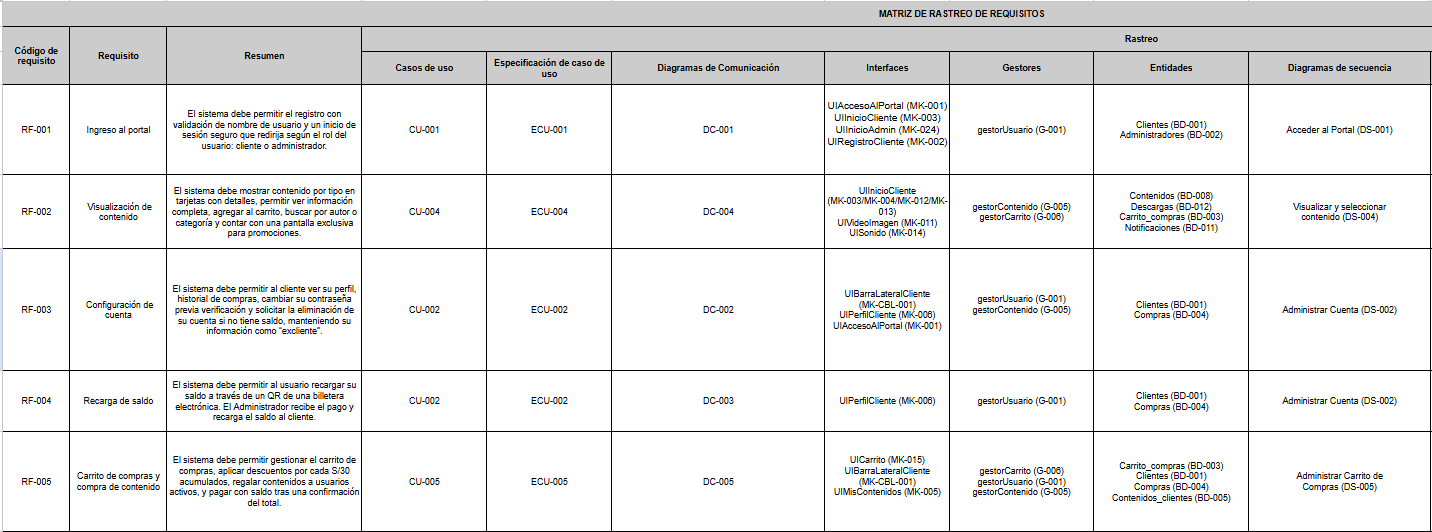
\includegraphics[width=1.1\textwidth]{Media/2_SeccionAdministrativa/MatrizRastreo.png}
    \caption{Vista previa de la matriz de rastreo de requisitos} 
    \label{fig:MatrizRastreo}
\end{figure}

\textbf{Link de la matriz de rastreo de requisitos:} \linkMatrizRastreo \\
